\begin{frame}
	\frametitle{Sharing Economy}

	\begin{itemize}
		\item Dienstleistung
		\item Vernetzen
		\item Besitz teilen
		\item Kosten verringern
	\end{itemize}
\end{frame}
\note{Kern ist immer eine Dienstleistung}

\begin{frame}
	\frametitle{P2P Platform Model}

	\begin{figure}
		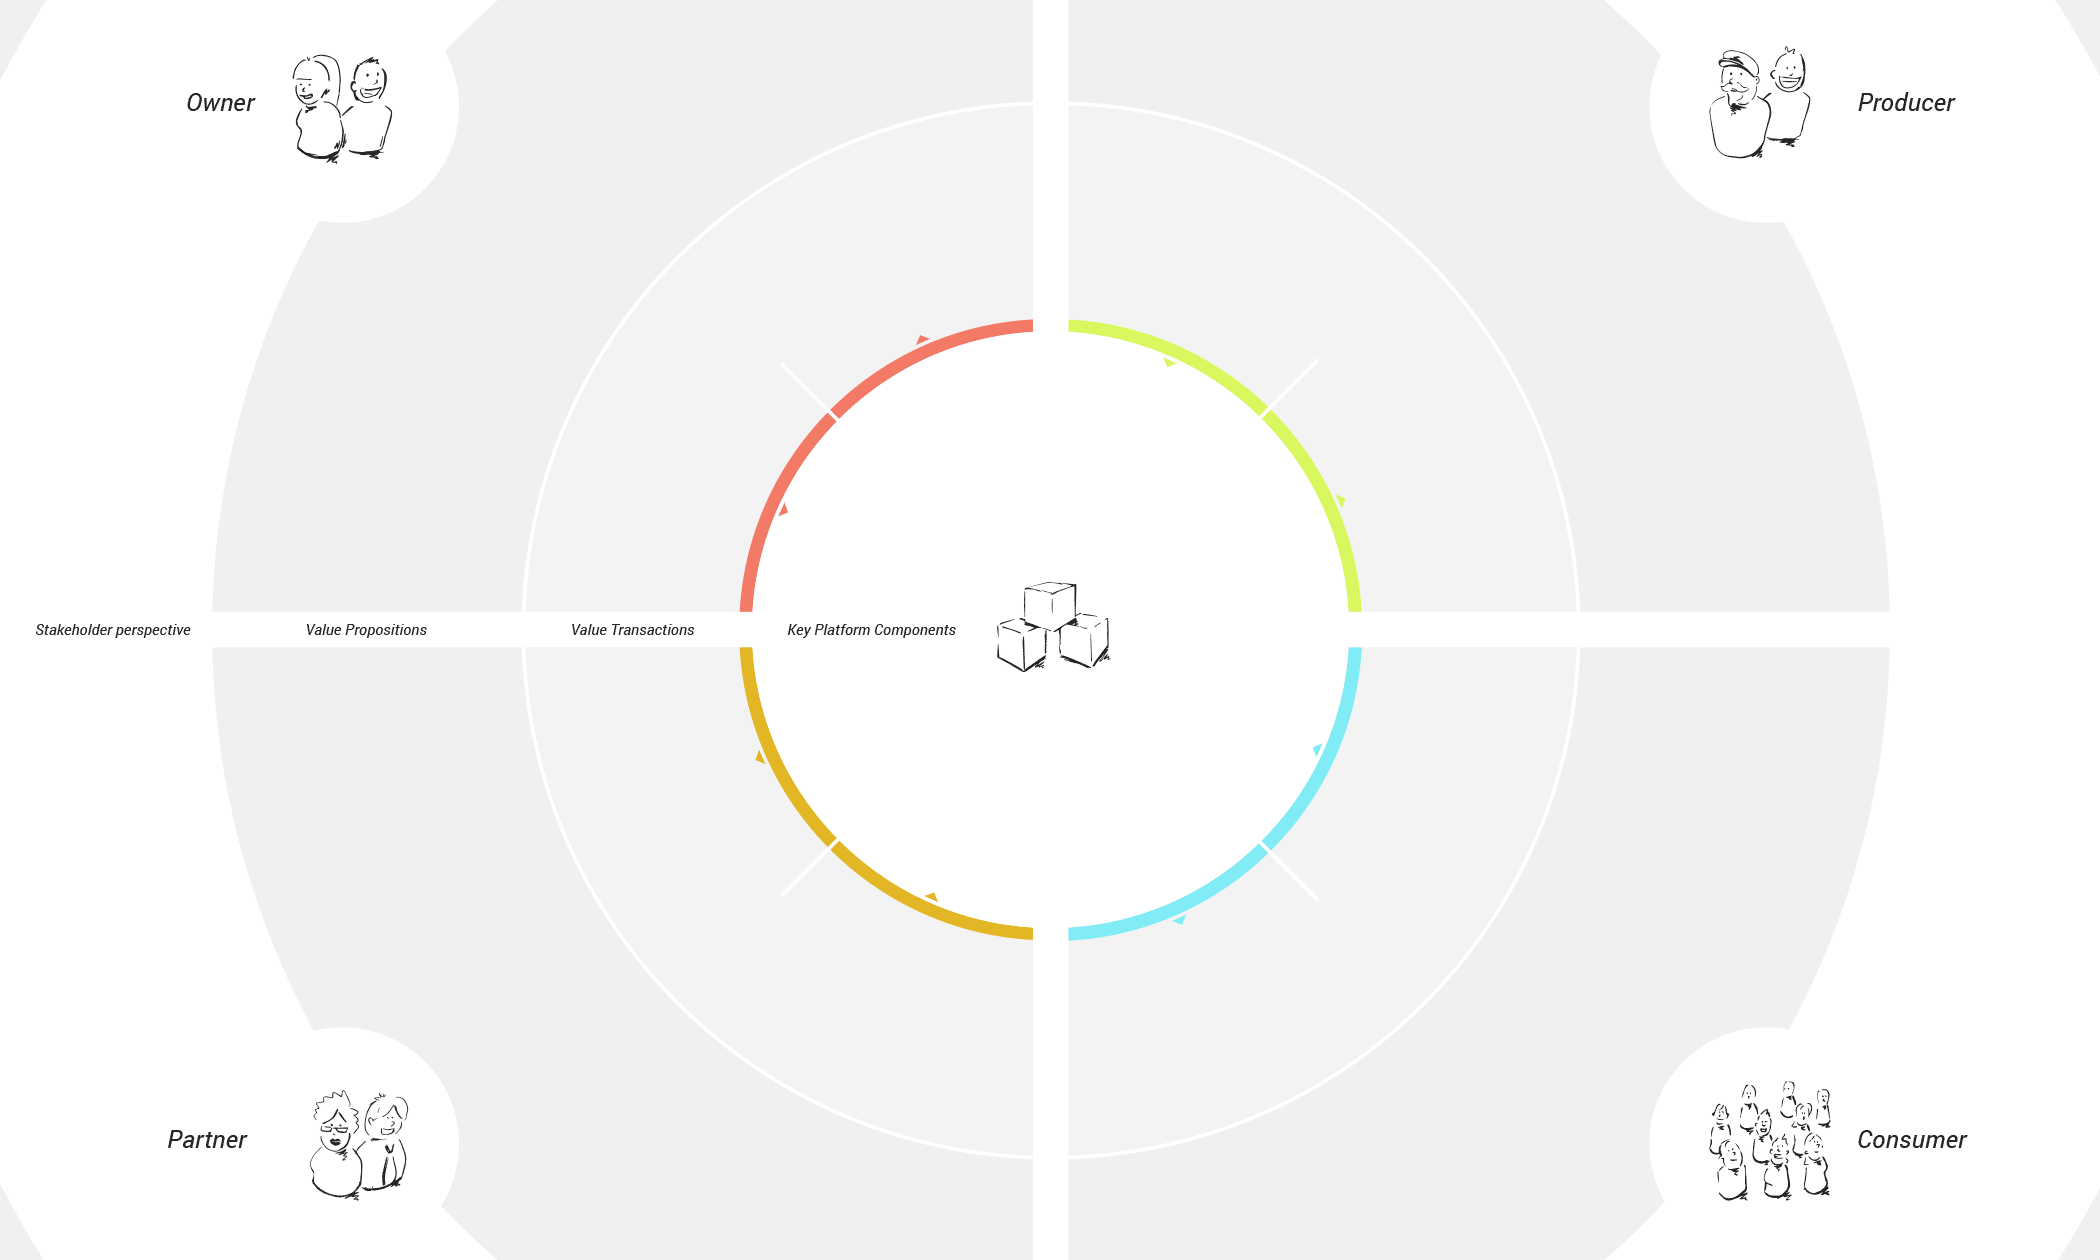
\includegraphics[height=0.8\textheight]{img/platformbusinessmodelcanvas.png}
		\caption[Platform Business Model Canvas]{\href{https://www.creatlr.com/template/um2yxrXADndCd8ftsGgY2/platform-business-model-canvas/}{{Platform Business Model Canvas}, Digital Ahead, \href{http://creativecommons.org/licenses/by-sa/4.0/}{CC BY-SA 4.0}}}
	\end{figure}
\end{frame}
\note{}

\begin{frame}
	\frametitle{Beispiel: Airbnb}

	\begin{itemize}
		\item Consumer: Privatperson
		\item Producer: Privatperson
		\item Partner: Dienstleister
		\item Owner: Airbnb
		\item Core: Stay
	\end{itemize}
\end{frame}
\note{
In Berlin wird versucht mit der Begründung Wohnungsmangel dagegen vorzugehen; Hotels protestieren aber nicht in wahrnehmbarem Maße
}

\begin{frame}
	\frametitle{Beispiel: BlaBlaCar}

	\begin{itemize}
		\item Consumer: Privatperson
		\item Producer: Privatperson(?)
		\item Partner: Dienstleister
		\item Owner: BlaBlaCar
		\item Core: Ride, like hitchhiking
	\end{itemize}
\end{frame}
\note{Hat einzelne Platformen (wie Mitfahrgelegenheit, Mitfahrzentrale, … aufgekauft und eine europäische Platform angeboten statt einzelner nationaler.
Jetzt wird die Zahlung eingeführt und Märkte dazu wieder gespalten, nachdem die Konkurrenz ausgelöscht wurde. Machen Konsumenten das mit?
}

\begin{frame}
	\frametitle{Beispiel: Uber}

	\begin{itemize}
		\item Consumer: Privatperson
		\item Producer: Privatperson(?)
		\item Partner: Dienstleister
		\item Owner: Uber
		\item Core: Ride, service-oriented
	\end{itemize}
\end{frame}
\note{In Paris haben Taxi-Fahrer Uber-Autos angezündet und damit die Politik gezwungen ein Verbot auszusprechen;
In DEU haben die Taxifahrer bei der Politik gehör gefunden; parallel aber bieten Sie jetzt selbst Vereinfachungen und Integration an – weil sie die Unvermeidbarkeit erkennen
}

\begin{frame}
	\frametitle{Weitere Platformen}

	\begin{itemize}
		\item \href{http://www.snapgoods.com/}{snapgoods.com} 
		\item \href{https://www.teilauto.net/}{teilauto}
		\item \href{http://www.myhammer.co.uk/}{MyHammer}
		\item \href{https://fon.com/}{fon}
	\end{itemize}
\end{frame}
\note{
}
